\chapter{Heap Sort}

\section{Introduzione}
Introduciamo ora il terzo e ultimo algoritmo studiato, ovvero Heap Sort.

Esso è probabilmente uno dei migliori algoritmi di ordinamento, poiché ordina sul posto e la sua complessità asintotica massima è $T(n) = O(n\log n)$, quindi unisce i pregi di Insertion Sort e Merge Sort.

Il suo funzionamento è basato sugli alberi binari, più precisamente sugli alberi heap (da cui il nome dell'algoritmo).
Un albero max-heap (o min-heap) è un albero binario la cui radice è il nodo con chiave massima (o minima) rispetto a tutte le altre chiavi degli altri nodi. 

Usando questa importante proprietà, dopo aver reso l'array un albero max-heap con il metodo \verb|BuildMaxHeap|, possiamo estrarre un nodo alla volta dalla radice, richiamare il metodo \verb|MaxHeapify| sull'albero, estrarre la radice che sarà diventata di nuovo il nodo con chiave massima, e iterare fin tanto che l'albero non si svuota.

\section{Tempo di esecuzione}
Come abbiamo accennato nel paragrafo precedente, il tempo di esecuzione dell'algoritmo Heap Sort è $T(n) = O(n \log n)$, poiché sommiamo il tempo impiegato per eseguire $n$ volte \verb|MaxHeapify|, che è $O(n \log n)$, e il tempo impiegato per eseguire \verb|BuildMaxHeap|, che si dimostra essere $O(n)$. 

Sommando i due tempi, otteniamo un limite asintotico superiore $O(n \log n)$, che è quindi il tempo migliore rispetto a quelli di Insertion Sort e Merge Sort; a differenza di quest'ultimo, però, c'è una somma di due tempi, $n \log n$ e $n$, quindi all'atto pratico Heap Sort impiega un tempo quasi doppio di Merge Sort.

Come possiamo vedere nel grafico \ref{heap:fig}, il tempo di esecuzione cresce come $f(n) = a n \log n$, con $a = 2.5 * 10^{-5}$, coefficiente di crescita poco più piccolo del doppio del coefficiente $a = 1.5 * 10^{-5}$ trovato empiricamente nel Merge Sort.

\begin{figure}
	\centering
	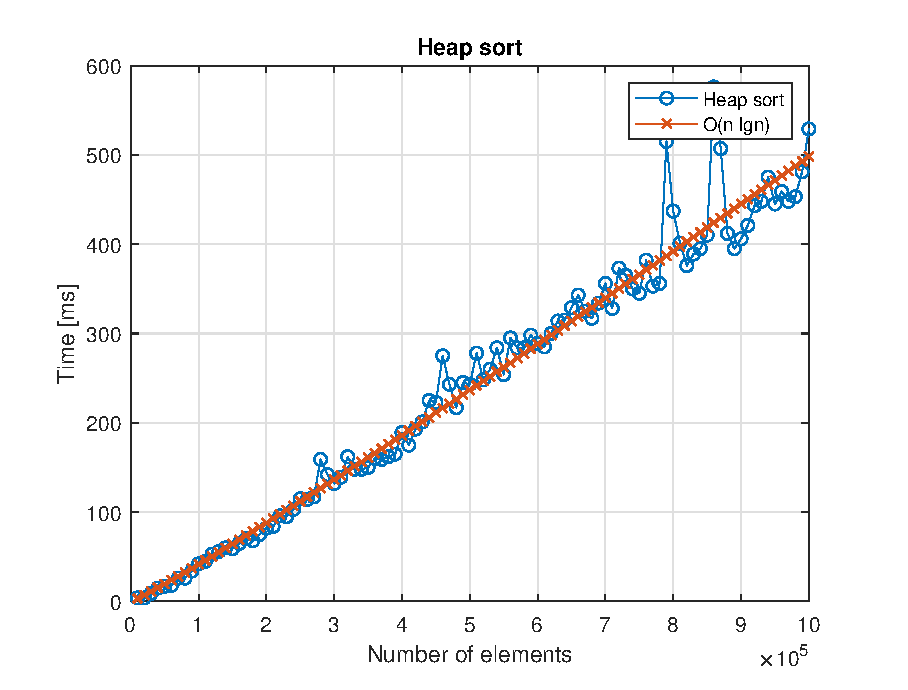
\includegraphics{./heap/graph.eps}
	\captionAlgorithm{Heap Sort}
	\label{heap:fig}
\end{figure} 